
\documentclass[12pt]{article}
\usepackage[margin=1in]{geometry}
\usepackage{amsmath}
\usepackage{setspace}
\usepackage{graphicx}
\usepackage{pdfpages}
\usepackage{float}
\graphicspath{ {images/} }
\begin{document}
\title{\centering Thesis Proposal:\\High Performance Finite Element Simulation for Soft Tissues}
\author{Haixiang Liu\\
University of Wisconsin, Madison\\
Advisor: Eftychios Sifakis}
\maketitle

\section{Introduction}

With the development of the theory of non-linear finite element and improvement of computation hardware, in recent years, using physics-based simulation for biomaterials became popular in biomechanics community in the examination of joint loading, tissue failures or for surgery prediction\cite{baldwin2012dynamic}\cite{tepole2014computational}\cite{rausch2016virtual}, etc. 

Soft tissues, including tendons, ligaments, blood vessels, skins or articular cartilages, and many others, serve important roles both biologically and mechanically. They bind, support, and protect the human body and structure. For instance, tendons connect bones and muscles to bones for stabilization or enabling motion. Ligaments connect bones to bones to restrict relative movement. Blood vessels distend in response to pulse waves. Skin is the largest organ supports internal organs and serve as a protective barrier that helps regulates heat and fluid loss, absorb shock and radiation etc. Articular cartilages exist as a 1-5mm layer on top of the joint connective parts to distribute load and reduce contact stress and friction\cite{holzapfel2001biomechanics}. 

Soft tissues are fibre-reinforced complex material. They mainly consist of a structural arrangement of collagen and elastin fibres that embedded in the hydrated matrix of proteoglycans. Their stress-strain response has been experimentally measured and categorized as highly non-linear and viscoelastic\cite{lanir1974two}\cite{mow1980biphasic}. 

Due to the complexity of the material properties, the finite analysis and simulation are conducted using commercially available softwares\cite{maas2012febio}\cite{hibbitt2001abaqus}. Those software though very robust in terms of supporting various constitutive models, but they require building explicit matrix when solving the system as a tradeoff and requires complex steps for setting up boundary conditions which limits their use to trained engineers. The long time for setup and running simulation makes it difficult for efficient clinical applications. As for the quality of discretization, those commercial softwares usually choose to use conforming tetrahedral or hexahedron mesh as their finite element. Even though those discretization elements can converge to continues solution at limit of refinement for the case of compressible isotropic linear elastic or Laplace equation. But they have known artifact for some problem that prevents the convergence. Locking, for instance, is the behaviour of the linear tetrahedral element exhibits a much higher stiffness due to the fact that the incompressibility of each element can impose much higher number of constraints than total degrees of freedom(*need a reference here*). As for hexahedron mesh the artifact of hourglass will be present when there is an insufficient quadrature rule is applied for element integration\cite{mcadams2011efficient}. We can see that the quality of discretization that whether it will converge to the continues solution and how fast it will converges is very much related to the constrain imposed by the constitutive model. While the present commercial FEM packages can not address such issue given their separation between discretization and constitutive modeling.

The simulation of soft tissue has also been of great interest in the field of virtual surgery. Either it is for training or for surgery planing, using accurate simulation can both reduce cost and decrease error. But in contrast to tissue analysis, virtual surgery applications require the simulation running at an interactive rate. Early works\cite{brown2001real}\cite{mollemans2003tetrahedral}, uses mass-spring system for simulation, though they can give fast simulation speed and benefits such as online cutting, a mass-spring system does not solve the underlining continuum equation correctly. In \cite{taylor2008high}, Taylor et al. proposed a GPU accelerated FEM simulator. Even though the system supports an anisotropic viscoelastic material model, the simulation was integrated explicitly for performance. GPU was also used for acceleration of the simulation in \cite{lapeer2011hyperelastic} by Lapeer et al. Three isotropic material models were considered along with mid point integration and the material parameters are fitted through experiments. The highest element count is 50,000 for this work. 

In another work by Mitchell et al.\cite{mitchell2015gridiron}, has used a non-conforming regular hexahedron grid and matrix free solver for better performance, that supports complex boundary conditions such as collisions. But only used single quadrature integration and limited to simple material models.

As for in the field of computer graphics, the use of physics based simulation to enhance animation has also attracted much attention and interest in the past decade\cite{mcadams2011efficient}\cite{kozlov2017enriching}\cite{sifakis2005automatic}. Due to the fact visual appearance is the only concern, those applications though were able to create visually convincing result by artists. They usually use very simple material model, lack validation, and trade fidelity with artistic control and performance.

Most of the work in graphics in skinning, for instance\cite{vaillant2014robust}, focus only on the surface. Even though it handles collision and has some quasi-elastic behavior and runs in realtime, it only creates plausible surface deformation of the skin and does not generate any dynamic secondary motion.

 Mcadam et al. in \cite{mcadams2011efficient}, proposed an efficient and stable single quadrature FEM simulation on a non-conforming Cartesian grid. Though the system has been used for simulating character anatomically\cite{milne2016flesh}, the material is limited to co-rotated linear elasticity. As in the goal of the system is to create efficient and simple way to generate contact collision and secondary motion in a believable fashion for animation, co-rotated linear elasticity is sufficient.
 
Among all the previous works, there is always the trade off between the performance and accuracy. For my thesis, using high-performance computing platforms, efficient data structure, high order finite element method, and accurate material model, I hope to engineer a solution for interactive high accuracy soft-tissue simulator.
 
 \section{Problems \& Challenges}
 
 In this section, I will describe the problems I intend to solve during the period of my Ph.D. study, what challenges they may impose, and finally the potential solutions to overcome them.

 \subsection{Discretization and data structure for efficient FEM simulation}
 
 \subsubsection*{Problem overview}
  
Traditionally there are three different discretizations for FEM simulation conforming mesh, non-conforming mesh, and meshless method. Conforming method means that the discretized solution space is a subset of the continues solution space. Even though conforming method can give more accurate result around boundaries without any special treatment, but constructing quality discrete conforming elements is both difficult and time-consuming in 3D. A poor quality mesh can cause the system to close to be singular and difficult to solve with limited floating point accuracy. Even with quality mesh, given the connectivity between elements of a conforming mesh is non-trivial, the neighboring information needs to be stored and can incur significant overhead in computation. 
 
Using non-conforming mesh, specifically surface embedding in a structured Cartesian grid, can be very efficient computationally, but regarding the boundary conditions, due to the fact that the discretized solution space is not a subset of the continues solution space, there can be large errors along the boundaries. Belyschko et al. \cite{belytschko2003structured} proposed an extended finite element method (X-FEM) and captures the surface by sampling point around the boundary and using radial basis functions to reconstruct the boundary equations. V.Kumar  et al.\cite{kumar2008implicit} used an level set representation of the surface and step functions for the basis of the elements at boundary. By doing so, captures the boundary condition exactly. Similarly in \cite{zhu2012second} a virtual node method was proposed for 2nd order accurate boundary condition capturing. But it was for linear elasticity. Another way to capture boundary conditions in a non-conforming simulation was proposed by Patterson et al. \cite{patterson2012simulation}. In this work, a monte-carlo sampling method was used to find the quadrature points for the integration within each boundary elements. To capture 2nd order accurate result, only 4 quadrature points were needed per element. But such method, even though highly efficient during the integration process, requires relatively expensive preprocessing time to find the quadrature points.

Another problem that rises with non-conforming mesh is embedding thin cuts in elements. Standard non-conforming mesh assumes continuity within element, while thin cuts within element would break such assumption. To overcome this issue method such as non-manifold level set representation of implicit surface combining with cut cell \cite{mitchell2015non} has been proposed.

(Still need to say something about meshless method (Or not....))

 \subsubsection*{Possible solutions}
 
For the reason of efficiency, I will focus on simulation in non-conforming mesh based methods using a regular Cartesian background grid. In \cite{setaluri2014spgrid}, Setaluri et al. proposed a novel data structure that utilizes the virtual memory system for efficient storage of sparse and adaptive grid data. It will be the primary data structure for storage. The adaptivity provided by SPGrid can also enable capturing high resolution and more local details. 

As stated in the overview, using non-conforming method will suffer from low accuracy along boundary and inability to capture thin cut features. To overcome those problem, I plan to use non-manifold level set proposed in \cite{mitchell2015non} as the storage for the implicit surface, and extended finite element method can be used along the boundaries to resolve boundary conditions. 

\subsubsection*{Challenges}

As mentioned in the introduction, discretization, as an estimation of the continuous equation, in an ideal case will converge to the continuous form of the solution under refinement. But in reality, under many cases, they exhibit different artifact based on the constraints imposed. It has been extensively studied for linear elasticity and other forms of PDE(*reference here*). But for nonlinear elasticity, there is very limited number of literature studied the discretization artifact for different constraints and there is very little understanding of the quality of discretization in this field. Many validations for the discretization are limited in single element test with prescribed affine transformation. Those tests can validate that the discretization equations are solved correctly, but are not sufficient in testing discretization artifact. In work \cite{zhu2012second}, Zhu et al. have used prescribed analytical deformations field to validate the 2nd order convergence rate of their discretization. But such technique only works for linear elasticity due to the uniqueness of the solution. For nonlinear elasticity, the solution may not be unique and a new verification technique is needed.

Biological soft tissues exhibit properties such as viscoelasticity, transversely isotropy, and highly non-linear strain-stress response\cite{holzapfel2001biomechanics}. Besides the challenge of finding suitable constitutive models that describe their mechanical behavior, there is the challenge of finding a proper efficient discretization and converges to the analytical expression of the constitutive model with refinement.

\subsection{Dynamic topology change}

\subsubsection*{Problem overview}
 
Either it is for surgical incision or for tissue failure under excessive tearing force, dynamic topology change during simulation is important for handling interactions with soft tissues and capturing their behaviour. Mesh cutting has always been considered a hard problem. After cutting, both the shapes of the elements and topology of the mesh will change. 

Many techniques have been developed for tetrahedral meshes. In work \cite{delingette1999hybrid}, the algorithm simply deletes the tetrahedral element that is been cut during simulation. Another work for cutting tetrahedral mesh was proposed by Sifakis et al. in \cite{sifakis2007arbitrary}. The authors proposed a robust cutting algorithm for tetrahedral meshes that with a high-resolution triangle surface meshes as the surface representation. Later Wang et al. have proposed another algorithm in \cite{wang2014adaptive}, what uses virtual node algorithm that can efficiently cut a tetrahedral mesh with a triangle surface. 

As for non-conforming FEM simulation with a hexahedron background grid, the elements of the background grid can not be cut into arbitrary shapes in comparison tetrahedral element simulation. But techniques, such as virtual node, discontinuous Galerkin method, and extended finite element can be used for dynamic cuttings of non-conforming FEM simulation. In work \cite{molino2005virtual}, 6 nodes were embedded in each tetrahedral mesh which allows a maximum of three cuts per element. Though the technique is developed for tetrahedral element mesh, using embedded nodes, we can also split a hexahedron element in a similar fashion. In \cite{kaufmann2009flexible}, Kaufmann et al. used discontinuous Galerkin method to support cuttings for hexahedron elements. But new hexahedron elements were created during the cutting due to the new degrees of freedoms introduced by the discontinuity at the cut. XFEM has been used to model structure fracture and cutting in the field of mechanical engineering for a long time. But mostly they are been used for rigid body or linear elasticity materials that undergo small deformation(*CITATION NEEDED*). Int \cite{jevrabkova2009stable}, Jer�bkov� et al. have proposed a fast and stable XFEM method for cutting nonlinear materials. But this work was also proposed for tetrahedral element meshes.

\subsubsection*{Challenges and Possible solutions}

Even though most techniques for cutting are developed for tetrahedral mesh simulation, they theory can potentially work for non-conforming mesh simulation with a hexahedron background grid with some adjustment. The virtual node algorithm and XFEM algorithms have been combined with hexahedron mesh for other features in literature. For instance, a second-order virtual node FEM algorithm has been combined with a 2D background grid in \cite{zhu2012second} for simulating nearly incompressible linear elasticity. In \cite{dolbow1999finite}, XFEM is proposed to model discontinuity(crack) in a hexahedron mesh with linear elasticity.
 
Whether it is virtual node algorithm or XFEM, in comparison to standard FEM algorithm, besides the extra computation, requires extra storage in the elements that contain discontinuity. To support online cutting or tearing, such storage must be able to grow with the simulation progress.
The virtual node algorithm, as presented in \cite{molino2005virtual}, has a maximum number of cuts supported per element. As for XFEM, it introduced a discontinuous shape function inside the element to model the cut. Standard 8 point Gauss quadrature rule works well for continuous shape function up to third order, but for a discontinuous shape function, a new integration method may need to be developed for accurate integration within an element.

\subsection{Vectorization and optimization for stream optimized platforms}

\subsubsection*{Problem overview}
 
Finite element simulations can be algorithmically formulated as sparse matrix operations or stencil operations. Those operations for each node only require information from a small surrounding region as input to compute the compute the output. Especially for non-conforming FEM simulation with a uniform hexahedron background grid, the sparsity patterns and stencils for each element are identical. Such characteristic exposes the opportunity to use SIMD (single instruction multiple data) hardware to speed up the performance of simulation. In recent years, SIMD hardware such as GPU or xeon Phi, features over 10 times more floating point operations per second (FLOPS) than traditional CPUs and 5 times more memory bandwidth. They have been used for physics based simulation for performance improvement for decades now. In \cite{mcadams2011efficient}, Mcadams et al. have used SSE instructions on CPU for data level parallelism, and achieved 3-7 times speed up using GPU. In \cite{mitchell2015gridiron}, Mitchell et al. have used the \textbf{Intel Xeon Phi} hardware which features a 512-bit SIMD width for the FEM simulation.

\subsubsection*{Challenges and possible solutions}
 
The first challenge a parallel algorithm faces is write-dependency. For FEM simulation, the computation usually involves reading nodal information and compute the contribution of each element and accumulate back to the nodes. But each node is shared by many elements. To prevent the situation of many threads computing different elements writing back to the same node, the final accumulation operation cannot be safely executed without a lock. But frequent locking can be extremely expensive and easily become the bottleneck of the computation. In \cite{mcadams2011efficient}, Mcadams et al. used a two pass algorithm to avoid such write dependency. First, a cell center stress value was computed in the first pass, then the nodal force was computed by taking the divergence of the adjacent cell stresses without the need of the accumulation operation. But this solution is very specific to the constitutive and single point integration scheme of their choice. Another potential solution for eliminating the accumulation operation is to do duplicated computation, instead of split elements to threads, we can split nodes to threads, and for each node, we compute the force contributing of all elements that contain this node. A limitation to this strategy is, even though the write dependency is eliminated, a significantly more amount of computation is needed, for each element not is computed many times.
 
.....MORE HERE....

\subsection{Constitutive models selections and validation}

\subsubsection*{Problem overview}

Biological soft tissues exhibit mechanical properties such as non-linearity, and anisotropy\cite{lanir1974two}, and viscoelasticity\cite{mow1980biphasic}. Many pieces of literature have proposed material models and parameters based on the experimental data. In general, there are two different approaches in picking or designing constitutive models: phenomenological and structurally based. (What is the definition of phenomenological constitute models?) Some of the examples phenomenological constitute models are: in work \cite{bischoff2000finite}, the skin is modeled as an isotropic non-linear hyperelastic material using the material model proposed by Arruda et al. in \cite{arruda1993three}. The parameters were fitted using an experimental result of a biaxial stretch test. In \cite{tepole2014computational}, In \cite{delalleau2006characterization}, Delalleau et al. used isotropic linear elasticity to estimate the parameter of the experimental result of an indentation test. In \cite {sun2005finite}, Sun et al. proposed a generalized Fung-elastic constitutive model that is based on the polynomial expansions of the entries of the strain tensor. On the side of the structural based constitutive modeling, soft tissues are considered to be an isotropic incompressible water-based matrix reinforced by a network of fibres. Tepole et al. In \cite{tepole2014computational} modeled skin as a isotropic Mooney-Rivlin hyperelastic material with a decoupled non-linear fibre term contribute to energy to capture the anisotropy. In \cite{gasser2006hyperelastic} Gasser et al. extended the idea of decoupling the single directional fibrous structure energy from the underlining matrix energy by introducing a fibre distributing function. There is no universally agreed constitutive model for soft tissues. Therefore, to be able to support many constitutive models is important in my exploration exploring the pro and cons for each constitutive model, and validate their quality in predicting mechanical properties of soft tissues.

\subsubsection*{Challenges and possible solutions}
 
 Though there are many attempts in proposing constitutive models for soft tissues. Many of them are designed and tuned to a very specific load test, for instance, uniaxial stress test, bi-axial stress, indentation test, etc. Even though the simulation of a given constitutive model with tuned parameter has matched the experimental data, there is no guarantee such model will predict the soft tissue behaviour under an arbitrary load. But it is difficult to setup experiments for arbitrary loads for the following several reasons. First, to tune the parameters or validate the constitutive model, both strain and stress field need to be measured. Most of the strain measurement can only record the strain field on the surface, but a vigorous validation would require the volumetric strain field as well. As for the stress measurement, usually, they are measured through a force sensor attached to a probe that applies stress to the specimen. Those probes have a limited degree of freedoms, and can't deform the specimen in arbitrary ways. Secondly, bio-tissues has a very limited period of viability, after several hours living bio-tissue will degenerate with a noticeable change of mechanical property. It is very difficult to perform several tests on the same specimen, and every specimen are unique due to the nature of the biological tissues. There is the possibility of using tissues from a cadaver. But those tissues are heavily processed and does not share the same mechanical properties as the living tissues in general.
 
Due to the constraints imposed by living tissues, for the scope of my study, I intend to use silicone rubber as a substitute. Such material has been used in surgical training and the field of special effect for many years. Even though silicone rubber has quite different mechanical properties than bio tissues, it has a highly non-linear response, (*\cite{martins2006comparative} READ THIS PAPER!!*) ..... and reproducible. With such material, I can use uniaxial stress test for parameter tuning, then validate the constitutive model and parameter with bi-axial stress and indentation test.
 
\section{Work to date}

\subsubsection*{A scalable Schur-complement fluids solver for heterogeneous compute platforms}

\begin{figure}[h]
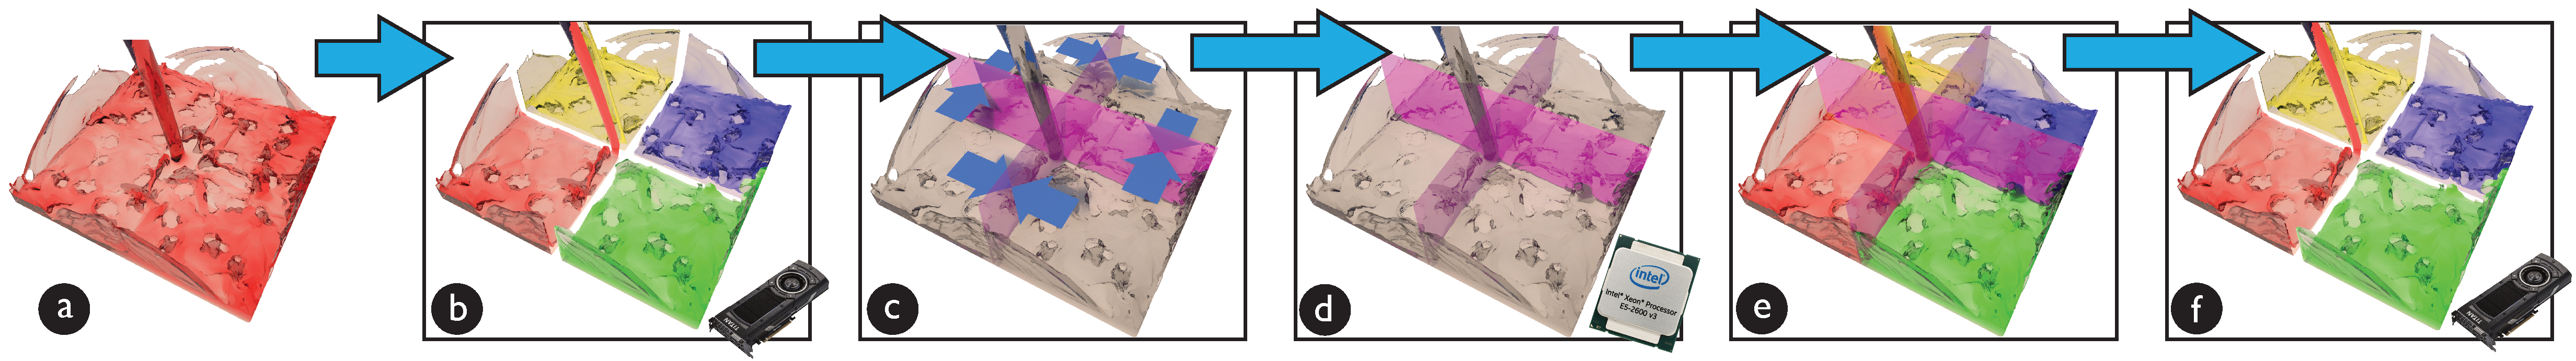
\includegraphics[width=\textwidth]{SolverStages.pdf}
\centering
\caption{Illustration of the core concept of our method: (b) We split the computational grid into subdomains, and independently solve them on the GPU(s), using zero Dirichlet conditions on subdomain boundaries. (c) Fluxes of the subdomain solutions are computed and sent to the CPU. (d) A specially formulated system is solved on the interface, using the CPU. This produces the exact value of the interface variables. (e) Those values are sent to the subdomains, and set as Dirichlet conditions. (e) A final subdomain solve on the GPU yields the global solution.}
\end{figure}
In work \cite{liu2016scalable}, my co-authors and I developed a solution for solving large scale finite difference Poisson problem in an efficient distributed fashion utilizing multiple stream optimized accelerators. The core contributing of the work is that we re-formulated the discrete Poisson problem into a collection of independent subdomain problems and a global interface problems that is the Schur-complement of the subdomains.

Each subdomain problem is solved based on the geometric multigrid algorithm proposed in \cite{mcadams2010parallel} by Mcadams et al.. Given that finite difference 3D Poisson problem is a uniform 7 point stencil operation, we utilized the high bandwidth and high computational throughput of stream optimized accelerators and created highly efficient subdomain solvers. 

As for the interface problem, in comparison to the subdomain problems, is highly irregular and, if written in explicit matrix form, a dense matrix operation while the subdomain problems are extremely sparse. To solve interface exactly would require super-linear complexity and it will easily be the bottle-neck of the solver. Instead of solving the interface exact, we proposed an approximate solver for the interface using an adaptive approximation and multigrid v cycle that executes in linear time with respect to the total number of degree of freedom on the interface. But as our solver by itself is only approximate, we used it as a pre-conditioner for the conjugate gradient method. As a whole, our iterative solver has linear complexity per iteration and the number of iteration required to reduces residual in an order of magnitude is independent of the solution resolution.

\subsubsection*{Power Diagrams and Sparse Paged Grids for High Resolution Adaptive Liquids}

\begin{figure}[h]
\includegraphics[width=\textwidth]{power_diagrams_2017-10.png}
\centering
\caption{Close-up view of the simulation of a river flowing through a canyon. The adaptivity pattern, based on proximity to rigid boundaries, is shown along a vertical cross-section, on the right. A narrow band level set with resolution $2048^2$ x 4096 is used for interface tracking.}
\end{figure}

The work \cite{aanjaneya2017power} presented a 2nd order adaptive scheme for liquid simulation. The key contribution of this work is that a 2nd order pressure solver that allows interface cross different grid of different resolution. Previous adaptive methods on a regular grid either require refine surface of the liquid completely and change grid topology every time step\cite{losasso2004simulating}, or only achieved 1st order accuracy along grid resolution changes\cite{losasso2006spatially}. To achieve 2nd order accuracy cross grid resolution, we combined the data structure of SPGrid \cite{setaluri2014spgrid} and power diagram \cite{de2015power} and developed a new fast marching and advection scheme. 

\subsubsection*{Efficient Elasticity for Character Flesh Simulation on Octrees}

This is the project I was working on during my internship with Disney Animation Studio in the summer of 2016. It is currently under review of ACM Transactions on Graphics(?IS IT?). In this project, we extended the work\cite{mcadams2011efficient} by Mcadams et al. to using a adaptive grid for flesh simulation. In an animation production setting, the visual interests usually lies only on the surface. High resolution details underneath the surface are very costly to simulate and adds very little visual detail to the resulting character. We used a balanced linear octree as our main data structure. 

\section{Research Plan}

\bibliographystyle{unsrt}
\bibliography{ref}
\end{document}